\documentclass{beamer}

\usepackage[utf8]{inputenc}
\usepackage[T1]{fontenc}

\usepackage[english]{babel}
\usepackage{amsmath}
\usepackage{cleveref}
\usepackage{amssymb}
\usepackage{mathtools}

%%Numbers, expectation
\newcommand{\N}{\mathbb{N}}
\newcommand{\E}{\mathbb{E}}
\renewcommand{\P}{\mathbb{P}}
\newcommand{\Var}{\mathbb{V}}
\newcommand{\R}{\mathbb{R}}
\newcommand{\D}{\mathcal{D}}
\newcommand{\B}{\mathcal{B}}
\newcommand{\Dh}{\D_h}
\renewcommand{\phi}{\varphi}
\newcommand*\diff{\mathop{}\!\mathrm{d}} % integral

%% mathoperator
\DeclareMathOperator*{\argmax}{arg\,max}
\DeclareMathOperator*{\argmin}{arg\,min}
\DeclareMathOperator*{\dom}{dom}
\DeclareMathOperator*{\sign}{sign}
\DeclareMathOperator*{\diag}{diag}

\DeclareMathOperator*{\Cov}{Cov}
\DeclareMathOperator*{\Cor}{Corr}
\DeclareMathOperator*{\Id}{Id}

%proximal operator
\newcommand{\prox}[3][]{\operatorname{prox}^{#1}_{#2}\left(#3 \right)}

\usepackage{xcolor}

%% sort citations by increasing number
\usepackage[sort,nocompress]{cite}

\usepackage{graphicx}% http://ctan.org/pkg/graphicx
\graphicspath{{../figures/}{../../figures}{../../memes}} %Setting the graphicspath
\usepackage{caption,subcaption}

\usepackage{tikz}
\usepackage{pgfplots}
\usetikzlibrary{backgrounds}
\usetikzlibrary{intersections}
\usepgfplotslibrary{fillbetween}

% \usepackage[right]{showlabels}


%%
\theoremstyle{plain}
\newtheorem{prop}{Proposition}[section]
\newtheorem{algo}{Algorithm}[section]
\newtheorem{assumption}{Assumption}
\theoremstyle{remark}
\newtheorem{remark}{Remark}[section]

% cref
\crefname{assumption}{Assumption}{Assumptions}
\crefname{equation}{}{}

\usepackage{autonum}

\usepackage{bm} %% bold math symbols

\usepackage{bbm} %% for \mathbbm{1}


% algorithmic environment
\usepackage{algorithm}
\usepackage[noend]{algpseudocode}

% for some reason this was required on one void linux installation (but not the other)
\usepackage{sansmathaccent}
\pdfmapfile{+sansmathaccent.map}

\author{Axel Böhm}

% shows which section we're in
\usetheme{Darmstadt}

% page number
\setbeamertemplate{footline}[frame number]
\setbeamercolor{page number in head/foot}{fg=gray}


% display things like onslide or visible already before but grayed out
\setbeamercovered{transparent}

% set the itemize item symbol as a diamond
\setbeamertemplate{itemize item}{$\diamond$}
% set the itemize subitem symbol as a triangle
\setbeamertemplate{itemize subitem}{$\blacktriangleright$}

% set the enumerate item symbol as a roman numbers
\setbeamertemplate{enumerate item}{(\roman{enumi})}


\author{Axel Böhm}

% shows which section we're in
\usetheme{Darmstadt}

% page number
\setbeamertemplate{footline}[frame number]
\setbeamercolor{page number in head/foot}{fg=gray}


% display things like onslide or visible already before but grayed out
\setbeamercovered{transparent}

% set the itemize item symbol as a diamond
\setbeamertemplate{itemize item}{$\diamond$}
% set the itemize subitem symbol as a triangle
\setbeamertemplate{itemize subitem}{$\blacktriangleright$}

% set the enumerate item symbol as a roman numbers
\setbeamertemplate{enumerate item}{(\roman{enumi})}


\title{Projected Gradient Descent}
\date{\today}

\begin{document}
\maketitle
\frame{\tableofcontents}

\section{Introduction}%



\begin{frame}
  \frametitle{Constrained Optimization}

  \begin{minipage}{0.5\textwidth}
    \begin{block}{Constrained optimization problem}
      \begin{equation}
        \begin{aligned}
          \text{minimize} & f(x)\\
          \text{subject to } & x\in C
        \end{aligned}
      \end{equation}
      \textcolor{blue}{How to solve them}
      \begin{itemize}
        \item Project onto $C$
        \item transform to \textit{unconstrained problem}
      \end{itemize}
    \end{block}
  \end{minipage}
  \begin{minipage}{0.45\textwidth}
    \begin{figure}[ht]
      \centering
      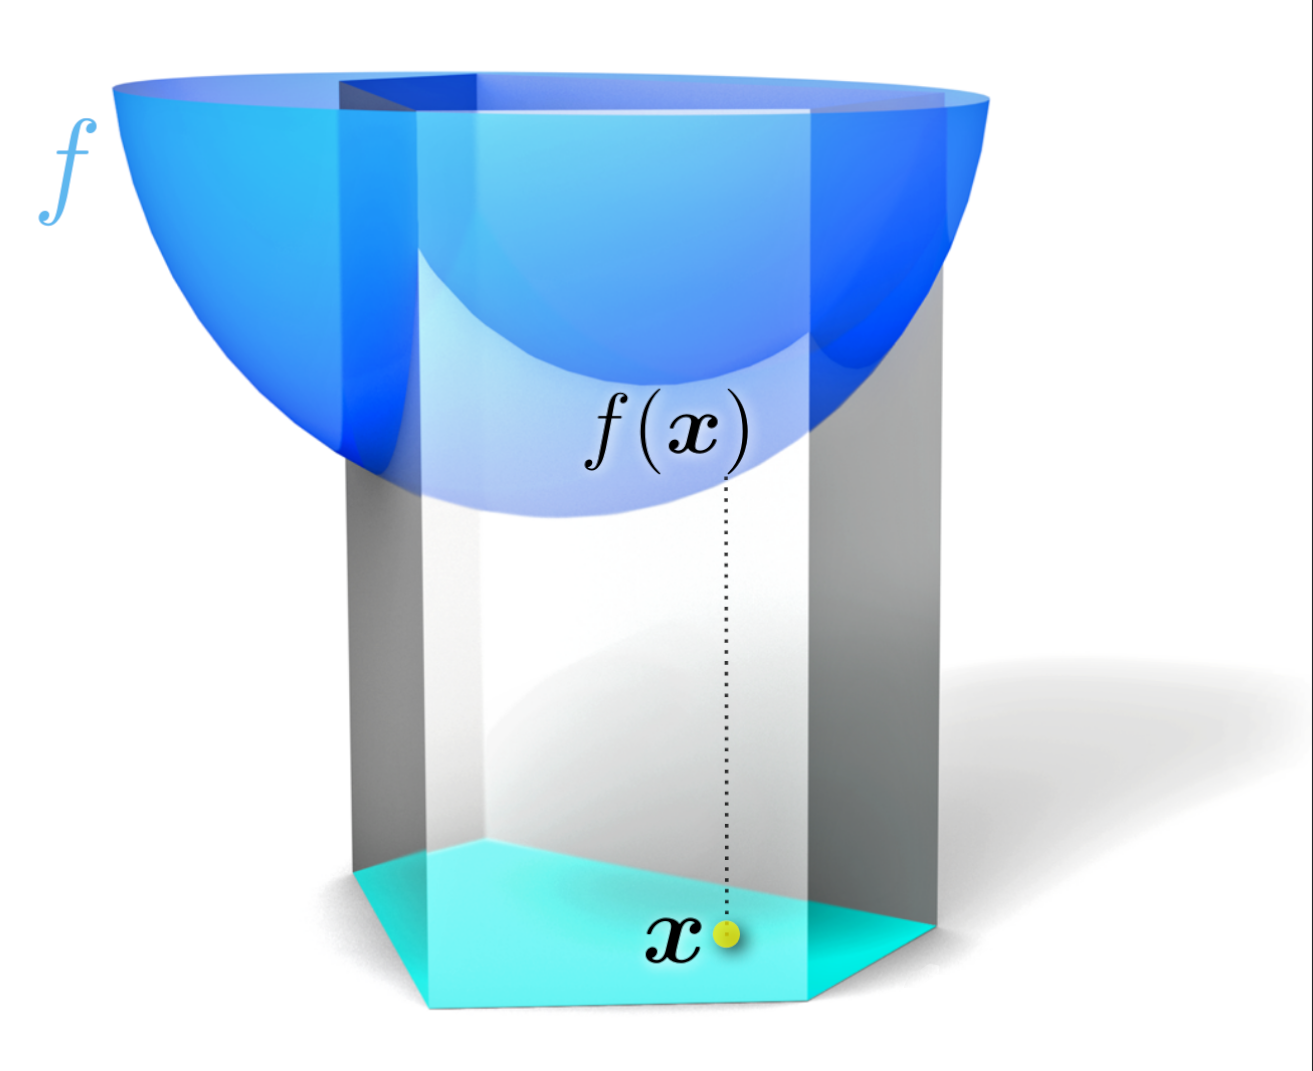
\includegraphics[width=\textwidth,height=\textheight,keepaspectratio]{constrained_3d}
      % \caption{\label{fig:label} }
    \end{figure}
  \end{minipage}
\end{frame}


\begin{frame}
  \frametitle{Constrained Optimization}

  \begin{minipage}{0.5\textwidth}
    \begin{block}{Constrained optimization problem}
      \begin{equation}
        \begin{aligned}
          \text{minimize} & f(x)\\
          \text{subject to } & x\in C
        \end{aligned}
      \end{equation}
      \end{block}
      \textcolor{blue}{We will focus on:}
      \begin{itemize}
        \item \textbf{Projected Gradient Descent}
      \end{itemize}
  \end{minipage}
  \begin{minipage}{0.45\textwidth}
    \begin{figure}[ht]
      \centering
      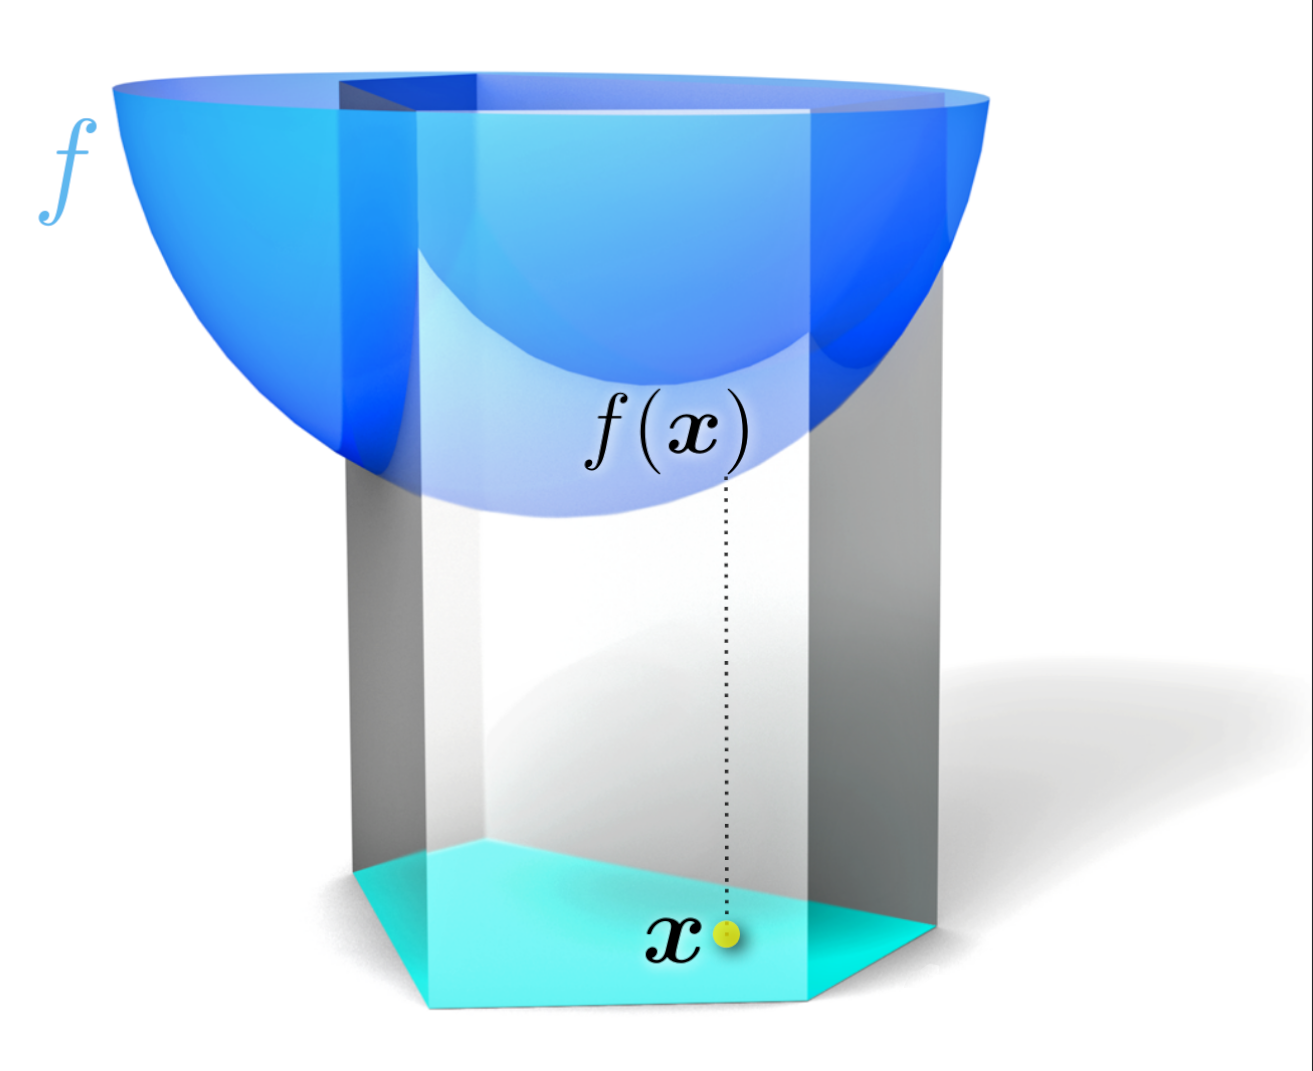
\includegraphics[width=\textwidth,height=\textheight,keepaspectratio]{constrained_3d}
      % \caption{\label{fig:label} }
    \end{figure}
  \end{minipage}
\end{frame}


\begin{frame}
  \frametitle{Projected Gradient Descent}

  % \begin{figure}[ht]
  %   \centering
  %   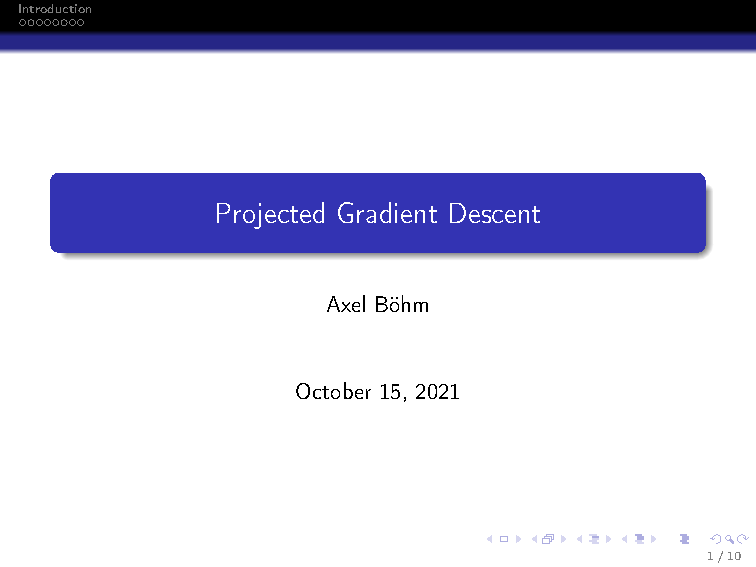
\includegraphics[width=\textwidth,height=\textheight,keepaspectratio]{projected_GD}
  %   % \caption{\label{fig:label} }
  % \end{figure}


\end{frame}


\begin{frame}
  \frametitle{Projected subgradient method}
  \begin{equation}
    \text{(constrained setting)} \quad \min_{x\in C}\, f(x)
  \end{equation}
  \begin{algorithm}[H]
    \caption{Projected subgradient method}\label{label:}
    \begin{algorithmic}[1]
      \For{$k=0, 1, \dots$}
      \State{Pick $g_k \in \partial f(x_k)$}
      \State{$x_{k+1} = P_C( x_k- \alpha g_k )$}
      \EndFor
    \end{algorithmic}
  \end{algorithm}
  By using the fact that the projection is a contraction
  \begin{equation}
    \Vert P_C(x) - P_C(y) \Vert \le \Vert x-y \Vert
  \end{equation}
\end{frame}

\begin{frame}
  \frametitle{Projected subgradient method II}
  \begin{proof}
    We can deduce the exact same inequality as before
    \begin{equation}
      \begin{aligned}
        \Vert x_{k+1} - x^* \Vert^2 &= \Vert P_C(x_k - \alpha g_k) - x^* \Vert^2 \\
        &\le \Vert x_k - \alpha g_k - x^* \Vert^2 \\
        &= \Vert x_k-x^* \Vert^2 + 2 \alpha \langle g_k, x^*-x_k \rangle + \alpha^2 \Vert g_k \Vert^2\\
        &\le \Vert x_k-x^* \Vert^2 + 2 \alpha (f^* - f(x_k))+ \alpha^2 \Vert g_k \Vert^2.
      \end{aligned}
    \end{equation}
  \end{proof}

\end{frame}




\end{document}
